\documentclass[11pt]{article}
\usepackage{amssymb}
\usepackage{amsmath}
\usepackage{multirow}
\usepackage{float}
\usepackage{url}
\usepackage{graphicx}
\usepackage{appendix}
\graphicspath{ {./images/} }

%Gummi|065|=)
\title{\textbf{To What Extent Have Techniques from the Fields of Number Theory and Algebra Been Useful in Attempting to Solve the Rational Cuboid Problem?}}
\author{Word Count: 3965}
\date{}
\begin{document}

\maketitle
\newpage
\tableofcontents
\newpage

\section{Introduction}
The Rational Cuboid Problem is an umbrella term used to refer to either partially or wholly rational cuboids, such as the Euler brick and the perfect cuboid. The perfect cuboid has rational edges and diagonals, including the space diagonal running through the body of the cuboid (Weisstein) \cite{perfectcuboid}. Variations of the rational cuboid problem remove some of the constraints on the perfect cuboid; for example, the Euler Brick problem does not necessitate a rational space diagonal. Common to these problems is the fact that they all form systems of simultaneous Diophantine equations which must be solved to give integer solutions.

This essay will explore a variety of techniques from the fields of number theory and abstract algebra and their use in making progress on the rational cuboid problem and its variations. The motivation for choosing these two fields results from the fact that Diophantine problems are inherently based in number theory, and the rational cuboid problem has direct links to Pythagorean triples, a concept with deep roots in number theory. Similarly, abstract algebra and algebraic number theory and geometry have a similar level of influence, as the structures encountered when assessing the properties and solutions of Diophantine systems feature heavily in those fields.

Techniques from these fields will be used to both find solutions to partially rational cuboids and further explore their properties as well as those of perfect cuboids, which remain insoluble.

\section{The Euler Brick Problem}
Consider a cuboid with sides $x$, $y$, and $z$ and face diagonals $d_1$, $d_2$, and $d_3$:

\begin{figure}[H]
\centering
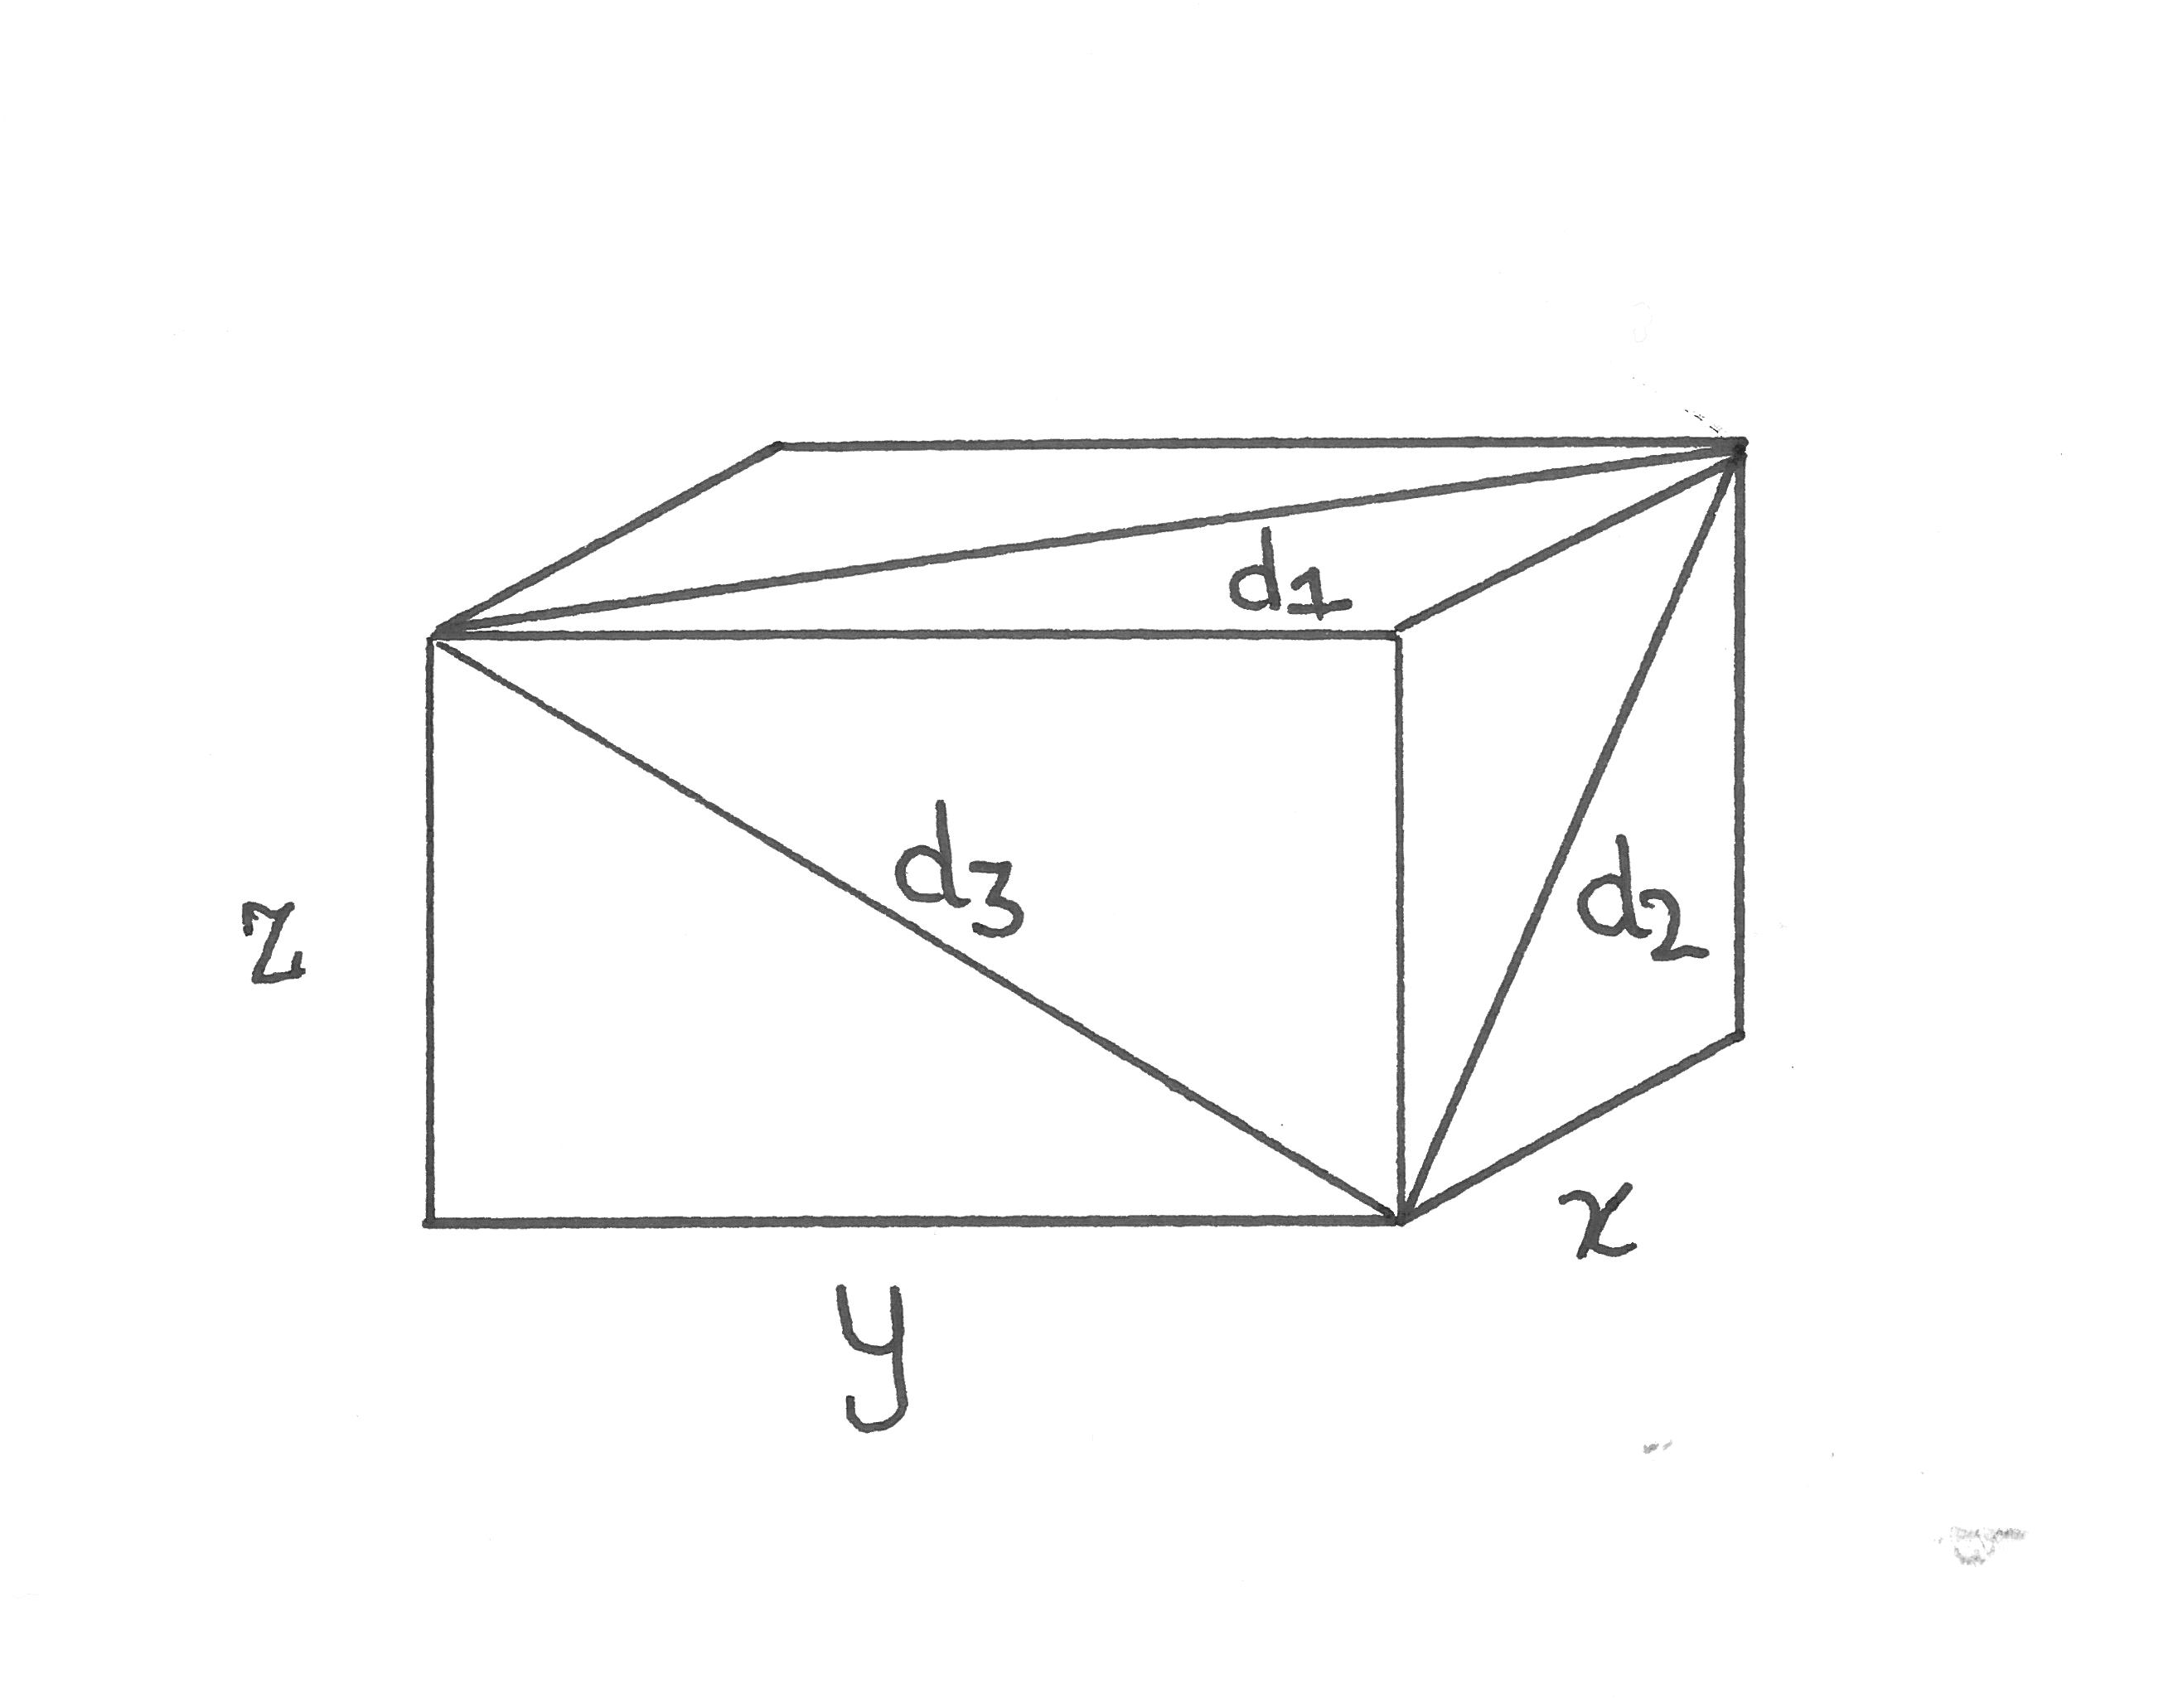
\includegraphics[scale=0.5]{1.png}
\end{figure}

Applying Pythagoras' theorem gives the following system of equations:
\begin{equation}
\begin{aligned}
x^2+y^2&=d_1^2 \\
x^2+z^2&=d_2^2 \\
y^2+z^2&=d_3^2 
\end{aligned}
\label{eq:1}
\end{equation}
In order for the cuboid to be an Euler brick, $(x, y, z)$ and $(d_1, d_2, d_3)$ must all be such that 
$${\{x, y, z, d_1, d_2, d_3\}}\subseteq{\mathbb{N}}.$$
This system of equations is referred to as a Diophantine problem, in this case with 3 equations in six variables. Note that the trivial solution of $(x, y, z)=(0, 0, 0)$ already exists, but we are only interested in primitive, nontrivial solutions. Nontrivial means that the solution is one that is not immediately obvious, while a primitive solution is one that can not be factorised into smaller solution (Weisstein) \cite{trivial}.

Since the equations concerning the Euler brick are Pythagorean triples, it makes sense to start by examining the properties of Pythagorean triples.

\section{Using Pythagorean triples}
\subsection{Euclid's Formula}
Consider a Pythagorean triple $a^2+b^2=c^2$. Rearranging,

\begin{equation*}
\begin{aligned}
a^2 &= c^2-b^2 \\
&= (c-b)(c+b).
\end{aligned}
\end{equation*}

The factors $(c-b)$ and $(c+b)$ must be square numbers in order for  $a$ to be a whole number. $c-b$ can therefore be expressed as $n^2$, where $n\in{\mathbb{N}}$.
Likewise, $c+b$ can be written as $m^2$, implying that $a=mn$.

Having expressed $a$ in terms of $n$ and $m$, the same can be done for $b$ and $c$.
$$(c-b)+(c+b)=2c$$
$$m^2+n^2=2c$$
$$\therefore c=\frac{m^2+n^2}{2}$$
Likewise for $b$,
$$(c+b)-(c+b)=2b$$
$$m^2-n^2=2b$$
$$\therefore b=\frac{m^2-n^2}{2}.$$
Simplified for convenience, 

\begin{equation}
\begin{aligned}
a &= 2mn     \qquad\qquad m, n \in{\mathbb{N}}\\\
b &= m^2-n^2 \\
c &= m^2+n^2.
\end{aligned}
\label{eq:2}
\end{equation}

This is Euclid's formula and allows for the generation of most Pythagorean triples (Joyce) \cite{euclidsformula}. Parameterising triples in terms of arbitrary numbers is beneficial as much of the mathematics concerning rational cuboids involves Pythagorean triples.

\subsection{Pythagorean Triples with Common Legs}
The method outlined below revolves around drawing a link between primitive Pythagorean triples with a shared leg.

In order for a Pythagorean triple ($x$, $y$, $d_1$) to be part of an Euler brick, $x$ and $y$ must both be part of two unique triples. As demonstrated in the previous section,
$$x^2=(d_1-y)(d_1+y)$$
Since $d_1-y$ and $d_1+y$ are two complementary factors of $x^2$, it follows that using varying pairs of values for either will yield different values for the other two legs of the triple, and thus multiple Pythagorean triples containing a common edge $x$. For example, $x^2=85^2=1^2\cdot{5}^2\cdot{17}^2$. Taking $d_1+y=25,$
$$85^2=25(d_1-y)$$
and $$d_1-y=289.$$
Adding and subtracting $d_1-y$ and $d_1+y$ gives $d_1=157$ and $y=132$. This gives a Pythagorean triple $(85, 132, 157)$, which fulfills the first equation, $x^2+y^2=d_1^2$. What must now be found is another Pythagorean triple containing the same $x$. This can be achieved by using the same approach as outlined above for the first triple, but with a different pair of factors. In this case, we can take $d_2+z$ to be $17\cdot{17}\cdot{5}$. Using this pair of factors gives $c=725$ and $b=720$, making a triple of $(85, 720, 725)$.

Up till now, the original system of Diophantine equations
$$x^2+y^2=d_1^2$$
$$x^2+z^2=d_2^2$$
$$y^2+z^2=d_3^2$$
is looking to be
$$85^2+132^2=157^2$$
$$85^2+720^2=725^2$$
$$y^2+z^2=d_3^2$$
Having found two triples with a common edge, there really isn't any choice with regards to the remaining triple, with the values of $y$ and $z$ having already been determined by the other two triples, in this case $132$ and $72$ respectively. An interesting consequence of this is that it implies that having an Euler brick that forms three primitive Pythagorean triples is impossible, as there must always be two even edges that form part of their own triple together. Another key thing to note is that this method relies upon trial-and-error for finding usable values of $a$. In the case of $a=85$, this happens to be the case as $132^2+720^2=732^2$ and we end up with an Euler brick of dimensions $(85, 132, 720)$. Letting $x=15$ also generates two unique Pythagorean triples, but the values of $y$ and $z$ produced by either don't form a triple themselves. 

The main takeaway here is that an Euler brick can be generated from an initial side length if and only if the side is part of two Pythagorean triples. The resulting condition for this is that the square of the side then be expressable in the form of two unique pairs of factors. The last condition is that the adjacent legs of those Pythagorean triples themselves form a triple, fulfilling the third equation in the set. Determining what initial values fulfill this property is where this method falls short, and the succeeding methods of parameterisation in the next section remedy this, mainly through defining the factor pairs in terms of arbitrary variables.
\section{Properties of the Euler Brick}
\subsection{Saunderson's Method}
One way of ensuring that Euler bricks are generated is by attempting to formalize the approach employed in the preceding section. As it turns out, this has already been done before with a parameterization having been developed by Nicholas Saunderson in the 16th century (Saunderson) \cite[p. 429-431]{saunderson}. Instead of relying upon partial trial and error or brute-force, using Saunderson's parameterisation allows us to generate an infinitude of Euler bricks from Pythagorean triples.

Given a primitive Pythagorean triple ($a$, $b$, $c$), an Euler brick with dimensions ($x$, $y$, $z$) can be generated as

$$x=4a^2b-c^2b,$$
$$y=4b^2a-c^2a,$$
$$z=4abc.$$

For example, the smallest Euler brick, with dimensions $(44, 117, 240)$, can be derived from the smallest Pythagorean triple $(3, 4, 5)$.

$$x=4\times{3^2}\times{4}-5^2\times{4}=44$$
$$y=4\times{4^2}\times{3}-5^2\times{3}=117$$
$$z=4\times{3}\times{4}\times{5}=240$$

The way Saunderson arrived at this parameterisation is fully discussed in Appendix A. In essence, Saunderson expressed the common even edge of two of the Pythagorean triples in terms of a pair of arbitrary sets of factors, which he then substituted back into the original equations in order to arrive at parameterised expressions for each edge of the Euler brick.


\subsection{Unparameterised Bricks}
The parameterisation given by Saunderson is not entirely comprehensive, meaning some Euler bricks cannot be parameterised. Indeed, the brick with dimensions $(85, 132, 720)$ from Section 3.2 cannot be reversed to give a Pythagorean triple. This can be explained in terms of the diagonals of the brick. 

Taking $x$ and $y$, the diagonal $d_1$ is given as
\begin{equation}
\notag
\begin{aligned}
d_1^2&=x^2+y^2\\
&=(4a^2b-c^2b)^2+(4b^2a-c^2a)^2\\
&=16a^4b^2+16b^4a^2-16a^2b^2c^2+c^6.
\end{aligned}
\end{equation}

However, $c^2=a^2+b^2$, and so
\begin{equation}
\notag
\begin{aligned}
d_1^2&=16a^4b^2+16b^4a^2-16a^2b^2(a^2+b^2)+c^6\\
&=16a^4b^2+16b^4a^2-16a^4b^2-16b^4a^2+c^6\\
&=c^6.
\end{aligned}
\end{equation}

From this, it can be seen that Saunderson's parameterisation produces integers that fulfill the two Diophantine equations $x^2+y^2=z^2$ and $x^2+y^2=z^6$. Alternatively, this can be seen as a requirement upon the generators $m$ and $n$ of $x$ and $y$, as $m^2+n^2=z^3$. 
One set of parametric solutions for the equation $x^2+y^2=z^6$ is given by: (Manasatarmgini) \cite{mana}

\begin{equation*}
\begin{aligned}
x&=2t^3+6t^2+3t-2, \\
y&=2t^3+12t^2+21t+11.
\end{aligned}
\end{equation*}

Setting $x=44$, one of the edges of the brick derived from Saunderson's parameterisation in Section 4.1, gives a value of $t=2$, which then gives $y=117$, corroborating with the actual dimensions of the brick. Since $t$ is required to be an integer, calculating $t$ for an edge of a non-Saunderson brick will give a non-integer value of t. This means that one can test whether a given Euler brick was generated by a Pythagorean triple by determining if the roots of the equation $2t^3+6t^2+3t-(2+x)=0$, where $x$ is one of the constant edge lengths of the brick, is whole.
For example, the brick with dimensions (85, 132, 720) cannot be parameterised since $2t^3+6t^2+3t-87=0$ gives $t=2.646$.

\subsection{Bricks with Edges of a Common Ratio}
Another question which naturally arises is the existence of Euler bricks that have two edges that reduce to the same ratio.
Intriguingly, this can be answered by examining a plane cubic curve in variables that denote the ratios between the generators of the individual triples in \eqref{eq:1}, an approach mentioned in brief by John Leech \cite{leech}.

Applying \eqref{eq:2} to each triple in \eqref{eq:1},

\begin{equation}
\begin{aligned}
x=2a_1b_1=a_3^2-b_3^2 \\
y=2a_2b_2=a_1^2-b_1^2 \\
z=2a_3b_3=a_2^2-b_2^2
\end{aligned}
\label{eq:4}
\end{equation}

Leech considers the ratios between these variables. In particular,
$$\frac{y}{x}\cdot\frac{z}{y}\cdot\frac{x}{z}=1,$$
and substituting different expressions for each occurrence of each variable gives
$$\frac{a_1^2-b_1^2}{2a_1b_1}\cdot\frac{a_2^2-b_2^2}{2a_2b_2}\cdot\frac{a_3^2-b_3^2}{2a_3b_3}=1.$$
In order to have opposite parity among the generators, which ensures primitivity, the first two fractions can be made so that
\begin{equation}
\frac{a_1^2-b_1^2}{2a_1b_1}\cdot\frac{a_2^2-b_2^2}{2a_2b_2}=\frac{\alpha^2-\beta^2}{2\alpha\beta}
\label{eq:5}
\end{equation}
The following algebra, attained through reversing the result obtained in \cite{leech}, aims to express \eqref{eq:5} in terms of the ratios $u=\frac{\alpha}{\beta}$ and $v=\frac{a_2}{b_2}$.
\begin{equation*}
\begin{aligned}
\frac{a_1^2-b_1^2}{2a_1b_1}&=\frac{\alpha^2-\beta^2}{2\alpha\beta}\cdot\frac{2a_2b_2}{a_2^2-b_2^2} \\
&=\left(\frac{\alpha^2-\beta^2}{\beta^2}\cdot\frac{\beta}{2\alpha}\right)\left(\frac{2a_2}{b_2}\cdot\frac{b_2^2}{a_2^2-b_2^2}\right) \\
&=\frac{\left(\frac{\alpha}{\beta}\right)^2-1}{\frac{2\alpha}{\beta}}\cdot{\frac{\frac{2a_2}{b_2}}{\left(\frac{a_2}{b_2}\right)^2-1}}
\end{aligned}
\end{equation*}
Substituting $u=\frac{\alpha}{\beta}$ and $v=\frac{a_2}{b_2}$, this gives
$$\frac{a_1^2-b_1^2}{2a_1b_1}=\frac{u^2-1}{2u}\cdot\frac{2v}{v^2-1}.$$
Letting $p=\frac{a_1^2-b_1^2}{2a_1b_1}$ for the sake of convenience and rearranging, we get
\begin{equation}
p(2u)(v^2-1)=(u^2-1)(2v).
\end{equation}
This equation is an algebraic cubic of the form $au(v^2-1)=bv(u^2-1)$, where $a$ and $b$ are constants in the field\footnote{A field is a set of numbers that is closed under the operations of addition and multiplication. Here, closure implies that any number generated by applying a binary operation such as addition or multiplication to pre-existing members of the field is a member of the field itself.} of rationals and $u$ and $v$ variables. An algebraic curve is the set of points for which some polynomial over a particular field equals zero, and the degree of the polynomial is the maximum degree of one of its terms (Weisstein) \cite{alcurve}. Since the terms $auv^2$ and $bu^2v$ have the highest degree of three, this curve is a cubic.

The constant $p$ represents the ratio of two edges $x$ and $y$ from any Euler brick. Since the equation is equivalent to \eqref{eq:5}, any rational points $(u, v)$ on the curve represent generators for an Euler brick with 2 edges in the ratio $p$. 

To illustrate, take the smallest Euler brick, (44, 117, 240). This brick involves three Pythagorean triples with three sets of generators as shown (the generators have been calculated using the method outlined in Appendix B):

\begin{table}[H]
	\centering
	\begin{tabular}{| c | c | c |}
		\hline
		Brick & Triple & Generators\\
		\hline \hline 
		\multirow{3}{*}{(44, 117, 240)} & (44, 117, 125) & {11, 2} \\ \cline{2-3}
		& (240, 117, 267) & {5, 8}  \\ \cline{2-3}
		& (44, 240, 244) & {5, 6} \\ \hline
	\end{tabular}
\end{table}

Taking the ratio of the legs of the last triple to be the constant $p$, Equation \eqref{eq:5} can be used to define a curve $F(x,y)=0$ where $F(x,y)=\frac{11}{60}\cdot(2x)(y^2-1)-(x^2-1)(2y)$:
\begin{figure}[h]
	\centering
	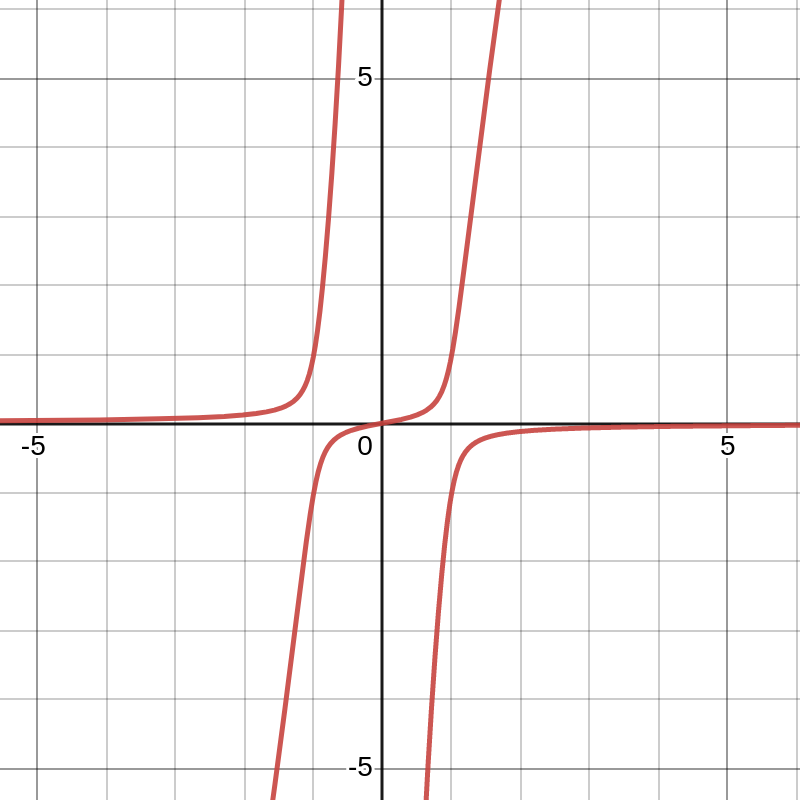
\includegraphics[scale=0.25]{4.png}
	\caption{The curve $\frac{11}{60}\cdot2x(y^2-1)-(x^2-1)(2y)=0$.}
\end{figure}

As mentioned, rational points on this curve signify Euler bricks with two sides in the ratio $11:60$, which is the same ratio as that of two sides from the brick (44, 117, 240). The point $P(\frac{8}{5},\frac{11}{2})$ for this brick is shown in Figure 2, and is one rational point on the curve. Since $F(x,y)=0$ is an algebraic cubic, rational points on its curve form a finitely generated abelian group\footnote{A group is similar to a field, but restricted to only one binary operation. Groups obey the axioms of closure, associativity, and the existence of an identity element and inverses (Foote), and an Abelian group has the additional property of the binary operation being commutative (Weisstein) \cite{axioms}\cite{abgroup}. The generators of a group are the elements of that group that can be used to generate all other elements by applying the binary operation to them. In the case of an algebraic cubic, any rational point acts as a generator, and since only one generator is thus required, the group is said to be finitely generated.}. This means that the group addition property for cubics can be used to find other rational points on the curve. If P is taken to be the sole generator of the set $C$ of points fulfilling $F(x,y)=0$ over $\mathbb{Q}$, then the point $2P$, obtained by applying the additive operation to $P$ itself, must also be in $C$ due to the closure property of groups. The additive operation for a single rational point, also referred to as a double point, is carried out by taking the tangent of the curve at the point and finding its point of intersection with the curve (Ash, Gross) \cite{elliptict}. Using implicit differentation, 
\begin{equation*}
\begin{aligned}
\frac{dF(x,y)}{dx}&=0 \\
\frac{11(y^2-1)}{30}+\frac{11x(\frac{dy}{dx}2y)}{30}-(4xy+2x^2\frac{dy}{dx}-2\frac{dy}{dx})&=0 \\
\frac{11(y^2-1)}{30}+\frac{11x(\frac{dy}{dx}2y)}{30}&=4xy+2x^2\frac{dy}{dx}-2\frac{dy}{dx} \\
11y^2-11+22xy\frac{dy}{dx}&=120xy+60x^2\frac{dy}{dx}-60\frac{dy}{dx} \\
\frac{dy}{dx}&=\frac{11y^2-120xy-11}{60x^2-60-22xy}.
\end{aligned}
\end{equation*}

At P, the gradient is thus $\frac{2937}{400}$, giving a tangent with the equation $y=\frac{2937}{400}x-\frac{781}{125}$:
\begin{figure}[H]
	\centering
	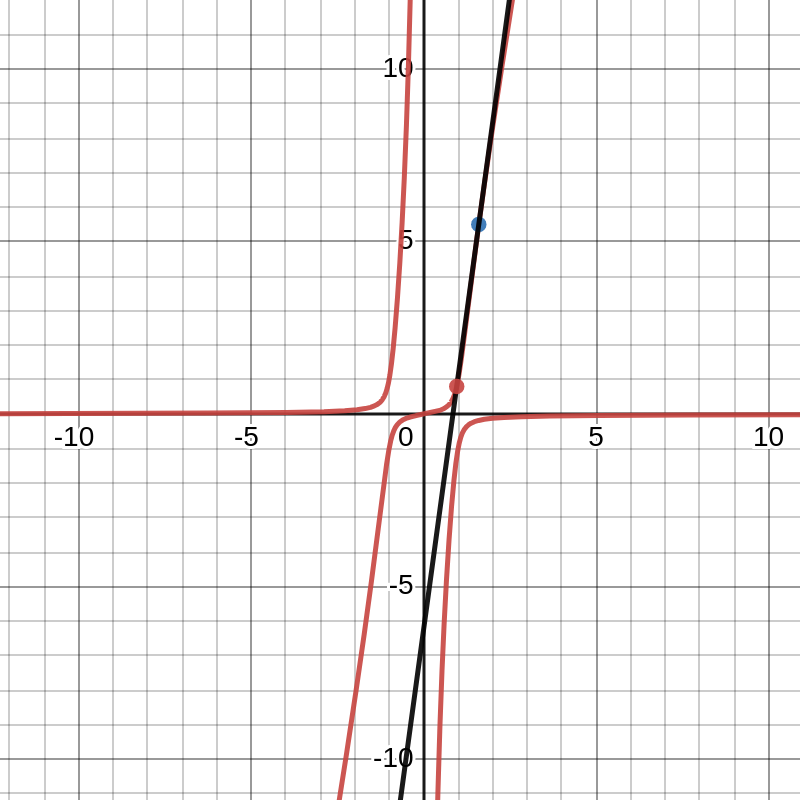
\includegraphics[scale=0.25]{5.png}
	\caption{The tangent at P and its two points of intersection with $F(x,y)=0$.}
\end{figure}

The tangent intersects the curve at the point $Q(\frac{10000}{10413}, \frac{3916}{4875})$. The individual coordinates of $Q$ are the ratios between the generators for the triples of the Euler brick with two sides in the ratio $11:60$. Take the brick to be (a, b, c). Then

\begin{equation*}
\begin{aligned}
a&=10413^2-10000^2=4875^2-3916^2=8430569, \\
b&=2(10413)(10000)=208260000, \\
c&=2(4875)(3916)=38181000, \\
\end{aligned}
\end{equation*}

and so the brick has dimensions (8430569, 208260000, 38181000). The ratio between $c$ and $b$ is $\frac{c}{b}=\frac{208260000}{38181000}=\frac{11}{60}$, which is the same ratio as that between the corresponding sides of the original cuboid. Other bricks with the same property can be found by finding more rational points on $F(x,y)=0$.


\section{Face Cuboids}
A face cuboid is defined by the set of equations
\begin{equation}
\begin{aligned}
x^2+y^2=d_1^2 \\
x^2+z^2=d_2^2 \\
x^2+y^2+z^2=d_4^2
\end{aligned}
\label{eq:6}
\end{equation}

A 3-orthoscheme is a tetrahedron with all four faces right-angled triangles, making it an equivalence to the right-angled triangle in three dimensions (Coxeter) \cite{coxeter}. Just as trirectangular tetrahedra are related to perfect cuboids (Section 7.3.1), 3-orthoschemes, also referred to as birectangular tetrahedra, are related to face cuboids.

Geometrically, birectangular tetrahedra are equivalent to face cuboids:

\begin{figure}[h]
\centering
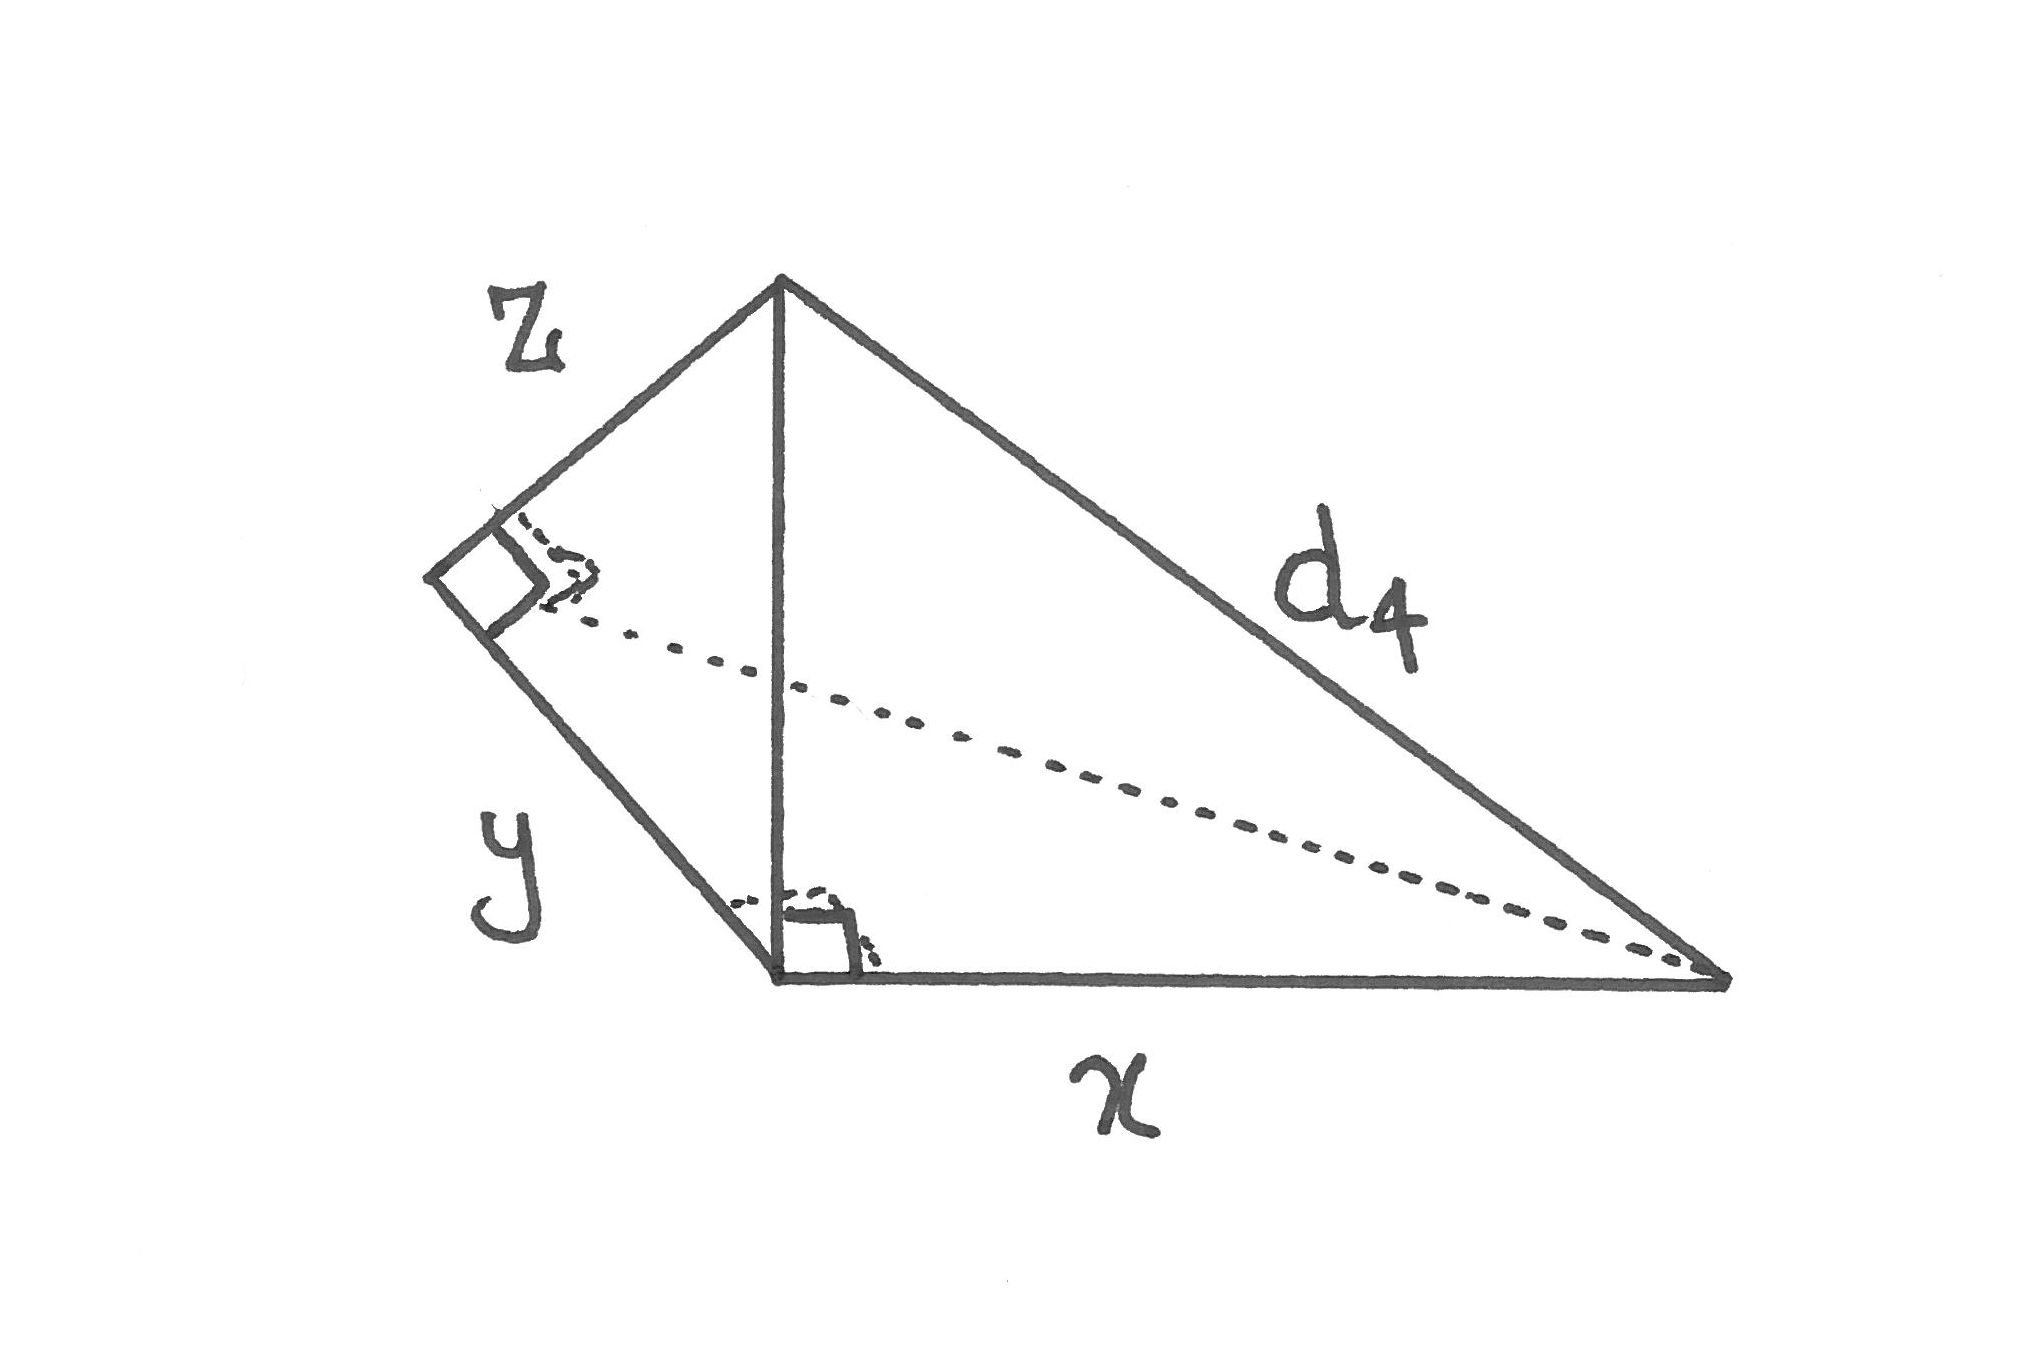
\includegraphics[scale=0.75]{6.png}
\end{figure}

Note that the first two equations in \eqref{eq:6} are the same as the first two for any rational cuboid, including the Euler brick. These equations ask for Pythagorean triples with a shared leg, the parameterisation for which has been derived independently in Appendix B.
By the parameterisation, the edges $x$, $y$, and $z$ are given as
$$x=2mnpq,$$
$$y=(mn)^2-(pq)^2,$$
$$z=(mp)^2-(qn)^2.$$

Substituting these values into the third criterion of \eqref{eq:6} gives the following condition on the four parameters $m, n, p,$ and $q$.
\begin{equation*}
\begin{aligned}
(2mnpq)^2+((mn)^2-(pq)^2)^2+((mp)^2-(qn)^2)^2&=\square \\
4m^2n^2p^2q^2+m^4n^4-2m^2n^2p^2q^2+p^4q^4+m^4p^4-2m^2p^2q^2n^2+q^4n^4&=\square \\
(mn)^4+(pq)^4+(qn)^4+(mp)^4&=\square \\
(m^4+q^4)(p^4+n^4)&=\square
\end{aligned}
\end{equation*}

Thus $(m^4+q^4)(p^4+n^4)$ must be a square number. For this to happen, either $m^4+q^4=p^4+n^4$ or $m^4+q^4=\square$ and $p^4+n^4=\square$.

For the former case, Euler gives the smallest possible solution as $m$=133, $n$=134, $p$=158, and $q$=59 (Euler) \cite{eulerface}. This gives a face cuboid with the dimensions (332273368, 230724000, 379083360).

Leech also discusses face cuboids, and gives a recursive formula for new pairs of generators and thus face cuboids \cite{leech}. This is obtained using a technique similar to that in Section 4.4; by considering the ratios between different variables in terms of their generator pairs.

Applying \eqref{eq:2}, the variables in \eqref{eq:6} can be expressed as

\begin{equation*}
\begin{aligned}
d_2&=\alpha_1^2-\beta_1^2=\alpha_2^2+\beta_2^2 \\
y&=2\alpha_1\beta_1=\alpha_3^2-\beta_3^2 \\
x&=2\alpha_2\beta_2=2\alpha_3\beta_3 \\
\end{aligned}
\end{equation*}

Since 
$$\frac{d_2}{y}\cdot\frac{y}{x}=\frac{d_2}{x},$$
\begin{equation}
\frac{\alpha_1^2-\beta_1^2}{2\alpha_1\beta_1}\cdot\frac{\alpha_3^2-\beta_3^2}{2\alpha_3\beta_3}=\frac{\alpha_2^2+\beta_2^2}{2\alpha_2\beta_2}
\label{eq:7}
\end{equation}

a recursive relationship can be derived by setting $u_i=\left(\frac{\alpha_i^2-\beta_i^2}{2\alpha_i\beta_i}\right)^2$. Another way of viewing this is by taking $u_i$ to be the ratio between the squares of the two legs of a Pythagorean triple generated by generators $\alpha_i$ and $\beta_i$. This has the benefit of allowing one to determine the third edge of a face cuboid knowing the other two using the recursive formula being derived.

The expression on the right hand side can be rewritten to express it in terms of $u_2$ through some manipulation:

\begin{equation*}
\begin{aligned}
u_2&=\left(\frac{\alpha_2^2-\beta_2^2}{2\alpha_2\beta_2}\right)^2 \\
u_2+\frac{4\alpha_2^2\beta_2^2}{4\alpha_2^2\beta_2^2}&=\frac{\alpha_2^4-2\alpha_2^2\beta_2^2+\beta_2^4}{4\alpha_2^2\beta_2^2}+\frac{4\alpha_2^2\beta_2^2}{4\alpha_2^2\beta_2^2} \\
&=\frac{\alpha_2^4+2\alpha_2^2\beta_2^2+\beta_2^4}{4\alpha_2^2\beta_2^2} \\
u_2+1&=\left(\frac{\alpha_2^2+\beta_2^2}{2\alpha_2\beta_2}\right)^2
\end{aligned}
\end{equation*}

Thus, (7) is equivalent to $u_1\cdot{u_3}=u_2+1$, which can be generalised to $u_i$:

\begin{equation}
u_{i-1}u_{i+1}=u_i+1
\end{equation}

Equation (8) is a Lyness cycle, a well known recurrence relation discovered by R.C Lyness \cite{lyness}. An interesting property of Lyness cycles is that they occur in cycles of 5, meaning that they have a period of 5 and repeat every 5 values. Thus, $u_{i+5}=u_i$. For brevity, this periodicity is demonstrating with arbitrary $u_1$ and $u_2$ in Appendix B.

Using the expressions for the individual terms of the Lyness cycle supplied in Appendix B, we can determine derivative face cuboids in terms of their originals. Given below is the Lyness cycle generated by $u_1$ and $u_2$ as defined prior.

\begin{equation*}
\begin{aligned}
u_1&=\left(\frac{\alpha_1^2-\beta_1^2}{2\alpha_1\beta_1}\right)^2=\left(\frac{d_2}{y}\right)^2 \\
u_2&=\left(\frac{\alpha_2^2-\beta_2^2}{2\alpha_2\beta_2}\right)^2=\left(\frac{z}{x}\right)^2 \\
u_3&=\frac{1+\left(\frac{z}{x}\right)^2}{\left(\frac{d_2}{y}\right)^2}=\frac{x^2+z^2}{x^2}\cdot\frac{y^2}{d_2^2}=\frac{y^2}{x^2} \\
u_4&=\frac{1+\left(\frac{y}{x}\right)^2}{\left(\frac{z}{x}\right)^2}=\frac{x^2+y^2}{x^2}\cdot\frac{x^2}{z^2}=\frac{d_1^2}{z^2} \\
u_5&=\frac{1+\left(\frac{d_1}{z}\right)^2}{\left(\frac{y}{x}\right)^2}=\frac{z^2+d_1^2}{z^2}\cdot\frac{x^2}{y^2}=\frac{(xd_4)^2}{(yz)^2}
\end{aligned}
\end{equation*}

Term $u_5$ gives one Pythagorean triple of the derived face cuboid:
\begin{equation*}
\begin{aligned}
(xd_4)^2+(yz)^2&=x^4+x^2y^2+x^2z^2+y^2z^2 \\
&=x^2(x^2+y^2)+z^2(x^2+y^2)=(x^2+z^2)(x^2+y^2) \\
&=(d_2d_1)^2
\end{aligned}
\end{equation*}

There is no apparent link between the Lyness cycle and the other two Pythagorean triples. Instead, they can be found by filling in the gaps. If we take $(d_2d_1)^2$ to be the leg of a Pythagorean triple itself, then multiplying $d_1$ by $y$ appears to give another leg that forms a triple with $(d_2d_1)^2$:

\begin{equation*}
\begin{aligned}
(d_2d_1)^2+(d_1y)^2&=x^4+x^2z^2+y^2x^2+y^2z^2+x^2y^2+y^4 \\
&=x^2(x^2+y^2+z^2)+y^2(x^2+y^2+z^2) \\
&=(d_1d_4)^2
\end{aligned}
\end{equation*}

Since the last triple is a basic triple with two squares and not three, and $(d_1y)^2$ must appear in two triples, it is given as:

\begin{equation*} 
\begin{aligned}
(d_1y)^2+(zy)^2&=(x^2+y^2)(y^2)+z^2y^2 \\
&=y^2(x^2+y^2+z^2) \\
&=(d_4y)^2
\end{aligned}
\end{equation*}

Thus, a face cuboid with dimensions ($x$, $y$, $z$) and diagonals ($d_1$, $d_2$, $d_4$) gives another cuboid with dimensions ($yz$, $yd_1$, $xd_4$). This formula can also be applied to itself to generate further face cuboids. However, instead of generating an infinity of cuboids, the 6th cuboid derived in such a manner is equivalent to the first, as evidenced by the links to the periodicity of the Lyness cycle through Equation \eqref{eq:7}. In this way, each primitive face cuboid can be considered to be the sole generator for a cyclic group\footnote{A cyclic group is a group generated by a single generator (Doer) \cite{cyclic}.} of face cuboids of order 5, thus forming another link to abstract algebra.

\section{The Perfect Cuboid}
Whereas the Euler brick only concerns the existence of a cuboid with integer edges and face diagonals, the perfect cuboid problem adds another condition; a rational body diagonal\cite{perfectcuboid}. This results in the introduction of another equation and hence another variable to the preceding system of equations for the Euler brick. This means that for a perfect cuboid with edges $x, y, z$,

$$x^2+y^2=d_1^2,$$
$$x^2+z^2=d_2^2,$$
$$y^2+z^2=d_3^2,$$
and \\
$$x^2+y^2+z^2=d_4^2,$$

where $d_4$ is the internal body diagonal of the cuboid. 

Unlike the Euler brick, no parameterisations exist for the perfect cuboid, and no perfect cuboids have been found through brute-force methods. However, this does not prove neither the existence nor the inexistence of a perfect cuboid, and hence this section will instead explore some properties of the perfect cuboid.

\section{Links between the Perfect Cuboid and Related Problems}

\subsection{Euler Bricks and Perfect Cuboids}
Can an Euler brick generated by Saunderson's parameterisation also be a Perfect Cuboid? The answer to this is unfortunately no.

For Saunderson's parameterisation, the body diagonal $d_4$ is given by
$$(4lmn)^2+(4n^2m-l^2m)^2+(4m^2n-l^2n)^2=d_4^2,$$
which simplifies to
\begin{equation}
m^6+19(m^2n^2)(m^2+n^2)+n^6=d_4^2.
\end{equation}
This gives a Diophantine equation in $m$, $n$, and $x$. Determining whether solutions exist can be done through modular congruences.

Two numbers $a$ and $b$ are congruent modulo another number $c$ if the remainder left upon dividing $a$ by $c$ is the same as that left by dividing $b$ by $c$. This equivalence between $a$ and $b$ is written as $a\equiv{b}\mod{c}$ (Weisstein) \cite{congruence}. For any $c$, the numbers that a square number $x$ can be congruent to modulo $c$ are called its quadratic residues (Ikenaga) \cite{residues}. For example, the quadratic residues for $c=8$ are 0, 1, and 4. In order to prove that a particular expression cannot be a square, its congruences modulo a particular number can be calculated and then compared with the quadratic residues for that number. If the congruences are not the same, then that expression can never be a perfect square. This logic can be applied to \eqref{eq:6} in order to determine whether the body diagonal of an Euler brick can ever be a perfect square. 

Usually, congruences are taken modulo powers of 2. Pocklington, who proves a generalised result for equations of this form, takes congruences modulo 16, and thus 16 is chosen here as well \cite{pocklington}. 

Since modular congruences can be added in the same way as normal numbers can, we can focus on the separate summands of the expression one at a time. By \eqref{eq:2}, the legs of a primitive Pythagorean triple must be of opposite parity. Since Saunderson's parameterisation requires that the parameters $m$ and $n$ form a Pythagorean triple, they must be of opposite parity. Setting $m=2k$ and $n=2l+1$, 
\begin{equation*}
\begin{aligned}
m^6+n^6&\equiv{64k^6+64l^6+6(2l)^5+15(2l)^4+20(2l)^3+15(2l)^2+6(2l)+1}\\
&\equiv{x}\mod{16}
\end{aligned}
\end{equation*}
through the binomial theorem, where $x$ stands for whatever numbers the square of the body diagonal is congruent to$\mod{16}$. By factoring 4 out,
$$4(16k^6+16l^6+6\cdot2^3\cdot{l^5}+15\cdot2^2\cdot{l^4}+20\cdot2\cdot{l^3}+15l^2+3l)+1\equiv{x}\mod{16}$$
This is an odd number of the form $4a+1$, and, as demonstrated in Appendix B, can be congruent to either 1, 5, 9, or 13$\mod{16}$.
As a result, 
$$m^6+n^6\equiv{1,5,9,13}\mod{16}.$$

Applying the same substitution to the rest of the expression, 
\begin{equation*}
\begin{aligned}
19(m^2n^2)(m^2+n^2)&\equiv{3((2k)^2(2l+1)^2)((2k)^2+(2l+1)^2)}\\
&\equiv{3(2k)^2(4l^2+4l+1)(4k^2+4l^2+4l+1)}\\
&\equiv{12k^2(4l^2+4l+1)(4k^2+4l^2+4l+1)\mod{16}}
\end{aligned}
\end{equation*}
(Note that the coefficient 19 changes to 3 as 19 reduces to 3 mod 16).

Note that $4k^2+4l^2+4l+1$ and $4l^2+4l+1$ are both odd numbers of the same form $4a+1$ discussed prior. Thus these two expressions are also congruent to 1, 5, 9, or 13 $\mod{16}$. This leaves $12k^2$. As we already know, $k^2\equiv{0,1,4,9}\mod{16}$, and so the congruence for the entire expression is given by the product of the individual congruences. Using the script from Appendix C for convenience, this ultimately gives $19(m^2n^2)(m^2+n^2)\equiv{0, 12}\mod{16}$.

Adding these congruences to those for $m^6+n^6$ has no effect upon them, as $x+0\equiv{x}\mod{16}$ and $12\equiv{-4}\mod{16}$, so that adding 12 to any of 1, 5, 9, or 13$\mod{16}$ simply gives another number already on the list. Consequently, 
$$d_4^2\equiv{1, 5, 9, 13}\mod{16}.$$
Since 5 and 13 are quadratic nonresidues mod 16, $d_4^2$ can never be a perfect square. Thus, modular congruences, which allow for one way of inspecting the properties of possible solutions, in this case the remainders left upon division by a particular number, can be used to determine whether solutions to particular Diophantine equations exist or not. Here, using modular congruences and basic modular arithmetic has demonstrated that no Euler brick produced from Saunderson's parameterisation can give a perfect cuboid.

\subsection{The Perfect Square Triangle Problem}
It is found that the perfect cuboid problem can be transformed into a variety of different problems, one of which is the perfect square triangle.

A perfect square triangle, while not formally defined, can be taken as a triangle with sides that are perfect squares, as well as rational angle bisectors. Florian Luca has demonstrated that a solution to the rational/perfect cuboid problem would result in a corresponding solution to a perfect square triangle, and vice versa, making the two equivalent \cite{luca}. The proof itself has been reproduced with some explanation in Appendix A.

An interesting corollary of this is that the perfect square triangle is also a Heronian triangle. A Heronian triangle is a triangle with an integer area as well as integer sides, and since $\sqrt{p(p-a)(p-b)(p-c)}$, which gives the area of the above triangle, is a perfect square, the perfect square triangle is also Heronian. Currently, the only known Heronian triangles with square sides are triangles with the sides $(1853^2, 4380^2, 4427^2)$ and $(11789^2, 68104^2, 68595^2)$ \cite{sqh1}\cite{sqh2}. Working back to obtain a cuboid by setting the sides to its face diagonals, it becomes apparent that neither of these is perfect square triangle. However, of interest is the fact that, for the first triangle, one of the edges is an integer with a value of $1387$, and for the second triangle, the corresponding cuboid has an integer body diagonal of $68595$. Unfortunately, for both, the rest of the edges are not whole numbers. 

\subsection{Heronian Tetrahedra}
Heronian tetrahedra are tetrahedra with sides, face areas, and volume all rational numbers. Since the former two criteria apply to the triangular faces of such tetrahedra, Heronian tetrahedra are composed of Heronian triangles. An interesting property of Heronian tetrahedra is that each example corresponds to an almost-perfect cuboid, one where all the edges, face, and body diagonals are integers bar one. In the case of Heronian tetrahedra, this is always one of the face diagonals. In order to see why this is so, we must first establish a link between Heronian tetrahedra and rational cuboids.

\subsubsection{Trirectangular tetrahedra}
If one were to take a cuboid and form a tetrahedron with the same dimensions, they would get a trirectangular tetrahedron, characterised by a vertex with three orthogonal edges and three right angles, all around the same vertex \cite{trirec}. All three faces with this shared vertex are then right-angled triangles, and the remaining face located opposite to the vertex can be referred to as the base. 
Since every cuboid has a corresponding trirectangular tetrahedron, and the Perfect Cuboid is a special case of a cuboid, the trirectangular tetrahedron produced by a perfect cuboid must also hold some unique properties. As it turns out, every tetrahedron with the same orthonormal sides as those of a cuboid must be Heronian. For a tetrahedron to be Heronian, it must have integer edges and face areas and an integer volume.
Consider a trirectangular tetrahedron with three orthonormal edges $x$, $y$, and $z$ that all obey (2).
By (2), this tetrahedron already has integer edges. The areas for all the right-angle faces are integers as well, as $A_r=\frac{xy}{2}$ where $x=2mn$ and $y=m^2-n^2$ for some $m$ and $n$, and the fact that one of the legs of a Pythagorean triple is always even means that dividing by two still gives a whole number. 
Calculating the base face area is slightly more involved. One way would be to use Heron's formula, which involves manipulating the semiperimeter of the base, i.e, the sum $\frac{d_1+d_2+d_3}{2}$, and makes for an unwieldy process. Another would be to use de Gua's theorem. De Gua's theorem, a generalisation of the Pythagorean theorem to the 3rd dimension, states that the square of the area of the base of a trirectangular tetrahedron is equal to the sum of the squares of the areas of its faces (Altshiller-Court) \cite{degua}:
$$A_B^2=A_1^2+A_2^2+A_3^2$$.
For the above tetrahedron, this gives the area of the base as
$$A_B=\frac{\sqrt{(xy)^2+(xz)^2+(zy)^2}}{2}$$
Unfortunately, this implies that a perfect cuboid and its corresponding tetrahedron will never have the same dimensions, as the above expression cannot equal a square under the sole premise of $x^2+y^2+z^2$ equalling a square. However, this does mean that a Heronian trirectangular tetrahedron with dimensions alike to (2) will yield a perfect cuboid with side lengths $2xy$, $2xz$, and $2yz$, since
$$(2xy)^2+(2xz)^2+(2yz)^2=A_B^2,$$
$$(2xy)^2+(2xz)^2=4x^2(y^2+z^2)=4x^2d_2^2=(2xd_2)^2,$$
$$(2xy)^2+(2yz)^2=4y^2(z^2+x^2)=4y^2d_3^2=(2yd_3)^2,$$
and
$$(2xz)^2+(2yz)^2=4z^2(x^2+y^2)=4z^2d_1^2=(2yd_1)^2.$$

\section{Conclusion}
Through exploring various versions of the rational cuboid problem, it has become apparent that both number theory and algebra have been very influential in both solving some problems as well as providing more insight into others. 

From the field of number theory, the concept of Pythagorean triples has played a very important role, largely owing to the fact that the equations concerning rational cuboids resemble systems of interrelated Pythagorean triples. In particular, the parameterisation of Pythagorean triples via Euclid's formula has been used to provide further parameterisations of simpler variants of the rational cuboid problem such as Euler Bricks and face cuboids through the consideration of shared edges. Examining the properties of the ratios between different variables has also allowed for links to be made with algebra. As well as this, the rational cuboid problem has also shown to be equivalent to special cases of Heronian triangles and tetrahedra through de Gua's theorem, a specialisation of the Pythagorean theorem to the third dimension. 

Links to algebra are made in the form of the face cuboid's representation as a Lyness cycle, which in turn has a cyclic group structure. As well as this, the use of algebraic cubics and the addition theorem for rational points allows for one to discern further properties of Euler bricks, such as the existence of bricks with sides in a common ratio.

Since the perfect cuboid problem does not resemble any similar form of Diophantine problem, there is no general technique to attempting it. In this regard, the use of algebraic geometry can prove useful, with algebraic varieties and their properties being particularly important with regards to providing insight into the constraints upon possible solutions.

\newpage
\bibliographystyle{ieeetr}
\bibliography{citation} 

\newpage
\begin{appendices}
	
\section{Derivations}
\label{appendix:misc}
\subsection{Saunderson's Parameterisation}
The derivation below has been interpreted from Saunderson's own notes \cite{saunderson}, but with added explanations and intermediate steps.

To start off with, instead of using actual values for the factors of $x^2$ as in Section 3.2, we can instead let there be two pairs of factors, defined as $(mk, \frac{x^2}{mk})$ and $(nk, \frac{x^2}{nk})$, which can be used in a similar manner to fill two of the three equations. Then, using the same properties of Pythagorean triples outlined earlier, the values of $y^2$ and $z^2$, which form the basis of the last remaining equation once the other two triples have been derived, are given as:
$$y^2=\frac{m^2k^2}{4}-\frac{x^2}{2}+\frac{x^4}{4m^2k^2}$$
and 
$$z^2=\frac{n^2k^2}{4}-\frac{x^2}{2}+\frac{x^4}{4n^2k^2}$$
The third equation in the system is $y^2+z^2=d_3^2$, which can now be given by 
$$d_3^2=\frac{m^2k^2}{4}-\frac{x^2}{2}+\frac{x^4}{4m^2k^2}+\frac{n^2k^2}{4}-\frac{x^2}{2}+\frac{x^4}{4n^2k^2}$$
$$=\frac{m^2k^2}{4}+\frac{n^2k^2}{4}-x^2+\frac{x^4}{4m^2z^2}+\frac{x^4}{4n^2z^2}$$
From here, utilizing the assumption that the above expression equates to a square number, we must find a way of expressing $x$, $y$, and $z$, i.e. the edges of the cuboid, in terms of the variables $m$ and $n$.

Looking at the sum of the first two terms of the expression, it is evident that the factors of $x$ $m$ and $n$ themselves form a Pythagorean triple, allowing for the introduction of a third variable $l$, defined as $\sqrt{m^2+n^2}$. In doing so, the sum of the first two terms can then be rewritten as
$$\frac{m^2k^2}{4}+\frac{n^2k^2}{4}=\frac{l^2k^2}{4}$$
In a similar fashion, the last two terms can be condensed into a singular expression involving $l$:
$$\frac{x^4}{4m^2k^2}+\frac{x^4}{4n^2k^2}=\frac{1}{4}\frac{x^4m^2+x^4n^2}{m^2n^2k^2}$$
$$=\frac{x^4l^2}{4m^2n^2k^2}$$
Ultimately yielding
$$d_3^2=\frac{l^2k^2}{4}-x^2+\frac{x^4l^2}{4m^2n^2k^2}$$
One way of fulfilling this equation, or, in essence, ensuring that the right-hand-side is a square number, is to make it such that the only term left is the very first one, which is guaranteed to be a square number. This simply means taking $d_3^2$ to be $\frac{l^2k^2}{4}$:
$$\frac{l^2k^2}{4}=\frac{l^2k^2}{4}-x^2+\frac{x^4l^2}{4m^2n^2k^2}$$
$$x^2=\frac{x^4l^2}{4m^2n^2k^2}$$
Simplifying further (dividing by $x^2$ and taking the square root), 
$$1=\frac{xl}{2mnk}$$
At this point, what we've managed to do is express one of our edges, $x$, in terms of factor pairs that assume separate variables. If we do the same with $y$ and $z$, the other two edges of the brick, we'll have successfully derived a parameterization of the Euler brick. 

Recall that we started off with assigning two different factor pairs to $x^2$, namely, $(mk, \frac{x^2}{mk})$ and $(nk, \frac{x^2}{nk})$. Also recall that, in the section prior, we derived multiple Pythagorean triples from a single $a$ using Euclid's formula. To recap, if $(a, b, c)$, arbitrary variables not in any way linked to the edges of our brick, form a Pythagorean triple,
then 
$$a=\sqrt{(c+b)(c-b)}$$
$$b=\frac{(c+b)-(c-b)}{2}$$
$$c=\frac{(c+b)+(c-b)}{2}$$
Since we have two factor pairs, we can have two separate forms of $a$, and for each form, it is the derivative value of $b$, or the shorter leg of the triangle formed by the consequent triple, that we are interested in, as opposed to the larger hypotenuse, or $c$, which would just give us one of the face diagonals of the brick as opposed to an edge.

Rearranging what we have up till now,
$$mk=\frac{xl}{2n}$$
and 
$$\frac{x^2}{mk}=x^2\cdot{\frac{2n}{xl}}=\frac{2nx}{l}$$
Since $mk$ and $\frac{x^2}{mk}$ are factors that multiply to give $x^2$, they can be rewritten in the form of $\sqrt{(c+b)(c-b)}$, and, working from this, we can then get a value of $y$, which shall be one of the edges of the brick. Taking $c+b$ to be $\frac{x^2}{mk}$ and $c-b$ to be $mk$, 
$$y=\frac{(c+b)-(c-b)}{2}$$
$$y=\frac{\frac{x^2}{mk}-mk}{2}$$
$$=\frac{\frac{2nx}{l}-\frac{xl}{2n}}{2}$$
$$=\frac{nx}{l}-\frac{xl}{4n}$$
Similarly, for the pair of factors $nk$ and $\frac{x^2}{nk}$, the resulting value of the side $z$ is $\frac{mx}{l}-\frac{xl}{4m}$.
Through this entire process, the sides of the brick $x$, $y$, and $z$ can now be written as
$$x=x$$
$$y=\frac{nx}{l}-\frac{xl}{4n}$$
$$z=\frac{mx}{l}-\frac{xl}{4m}$$
The last remaining step is to rewrite the starting value of the side $x$ in terms of the parameters $m, n,$ and $l$. Since $x$ is factored by all three and $x$ can be arbitrary anyhow, Saunderson chose to let $x$ equal $4lmn$, with the coefficient of 4 allowing for cancellation with any fractions.

As a result, the sides end up being:
$$x=4lmn$$
$$y=\frac{n\cdot{4lmn}}{l}-\frac{4lmn\cdot{l}}{4n}=4n^2m-l^2m$$
$$z=\frac{m\cdot{4lmn}}{l}-\frac{4lmn\cdot{l}}{4m}=4m^2n-l^2n$$

\subsection{Perfect Square Triangles and Perfect Cuboids}
Let $x, y, z$ be the edges of our theoretical perfect cuboid, and let $d_1, d_2, d_3$ be the face diagonals and $d_4$ be the body diagonal. Now, let $(a, b, c)=(d_1^2, d_2^2, d_3^2)\in{\mathbb{N}^3}$ for convenience. Since the sum of either two of $a, b,$ and $c$ is more than the remaining number, by the triangle equality, a triangle with sides that are perfect squares can be formed.

Now we let $p$ equal the semiperimeter of the triangle, so that $p=\frac{a+b+c}{2}$. The semiperimeter is simply half the perimeter of the triangle, and will be used to calculate the lengths of the angle bisectors of the triangle later on. The semiperimeter of this triangle is then equal to the square of the face diagonal of the original, theoretical perfect cuboid, since
$$p=\frac{a+b+c}{2}=\frac{d_1^2+d_2^2+d_3^2}{2}$$
$$=\frac{x^2+y^2+x^2+z^2+y^2+z^2}{2}$$
$$=x^2+y^2+z^2$$
which, owing to the fact that $x, y, z$ are sides of a perfect cuboid, equals the square of the face diagonal, $d_4$. Hence,
$$p=d_4^2$$
Now, the link between the perfect cuboid and the perfect square triangle is constructed through the fact that the square of the semiperimeter, which as we know must be a whole number owing to $p, d_4^2$ being square, is used to calculate the lengths of the angle bisectors of the triangle. In order to avoid further confusion by introducing new free variables to set an example, we shall instead demonstrate this on our perfect square triangle instead. 

The angle bisectors, or the lines that divide each angle of the triangle equally, are given as $l_a, l_b,$ and $l_c$ for angles opposite to sides $a, b,$ and $c$ respectively. Then, the lengths of these bisectors are given as
$$l_a=\frac{\sqrt{bcp(p-a)}}{b+c}$$
$$l_b=\frac{\sqrt{acp(p-b)}}{a+c}$$
$$l_c=\frac{\sqrt{abp(p-c)}}{a+b}$$
Since all the numbers forming the product inside the root of the numerator are square, it follows that the triangle must have rational angle bisectors with a whole numerator for each as defined above.

As a result, if a perfect cuboid does exist, then so does a perfect square triangle as outlined above. (Luca) \cite{luca}


\section{Demonstrations}
\label{appendix:par}
\subsection{Finding the Generators of a Pythagorean Triple}
Given a Pythagorean triple $(a,b,c)$, find $p, q$ such that $\frac{a}{b}=\frac{p}{q}$ in its simplest form. One of $p$ and $q$ will always be even. Taking $p$ to be even, set $p=2uv$ and $q=u^2-v^2$. Substituting $u=\frac{p}{2v}$ into $q$ yields a quadratic in $v^2$, which can then be solved to find $v$ and $u$, the generators of $(a,b,c)$.

\subsection{A Parameterisation for Pairs of Pythagorean Triples with a Shared Even Side}

For any Pythagorean triple, one of the sides can be given in terms of generators $u$ and $v$ as the product $2uv$. Since the other legs of the triple are dependent upon the values of $u$ and $v$, two triples with a same leg $a$ can only occur if $a$ can be expressed in the form $2uv$ for two different values of $u$ and $v$ each. 

If we let $u=mn$ and $v=pq$, then $a=2\cdot{mn}\cdot{pq}$ and part of the triple defined as
$$(2mnpq)^2+((mn)^2-(pq)^2)^2=((mn)^2+(pq)^2)^2.$$

However, $a=2\cdot{mn}\cdot{pq}=2\cdot{mp}\cdot{nq}$, and so $a$ is also part of the triple defined as
$$(2mnpq)^2+((mp)^2-(nq)^2)^2=((mp)^2+(nq)^2)^2,$$
making it part of two Pythagorean triples. Thus, any even number whose prime factorisation is expressible as four unique integers can be part of two Pythagorean triples.

\subsection{A Full Lyness Cycle}
Take $u_1=x$ and $u_2=y$. The recurrence relation between $u_n$, $u_{n+1}$, and $u_{n-1}$ is given by
$$u_{i+1}=\frac{1+u_i}{u_{i-1}}$$.
Then,
\begin{equation*}
\begin{aligned}
u_3&=\frac{1+y}{x}, \\
u_4&=\frac{\frac{1+y}{x}+1}{y}=\frac{1+x+y}{xy}\\
u_5&=\frac{1+\frac{1+x+y}{xy}}{\frac{x+y}{x}}=\frac{y(x+1)+x+1}{y(1+y)}\\
&=\frac{x+1}{y} \\
u_6&=\frac{1+\frac{x+1}{y}}{\frac{1+x+y}{xy}}=\frac{y+x+1}{y}\cdot\frac{xy}{1+x+y}\\
&=x=u_1
\end{aligned}
\end{equation*}

Thus, for all $u_n$, $u_n=u_k$ where $n\equiv{k}\mod 5$ and $k<5$.

\subsection{Odd Numbers of the Form 4n+1 mod 16}
For $n\leq{4}$, $4n\leq{16}$, and so $4n\equiv{0,4,8,12}\mod{16}$.

For $n>4$, $4n=4(4p+n-4p)=16p+4(n-4p)$. Since $4n>16$, $4n$ is the sum of a multiple of 16 plus a residual value, i.e., $4n=16k+x$, where $x<16$. Letting $p=x$ means that $n-4p\leq{4}$, and so $4n\equiv{16p+4k}\equiv{4k}\equiv{0,4,8,12}\mod{16}$, where $k=n-4p\leq{4}$.

For $4n+1$, 1 can be added to each congruence due to the fact that modular arithmetic operates in the same manner as normal arithmetic. Thus,
$$4n+1\equiv{1,5,9,13}\mod{16}$$

\section{Computer Scripts}

\subsection{Script to Combine Modular Congruences}
The Python 3 script below can be used to find sums or products of possible modular congruences:

\begin{verbatim}
def combine(n, l1, l2):
  congruences = []
  for i in l1:
    for j in l2:
      sum = i+j
      sum = sum % n
    if sum not in congruences:
      congruences.append(sum)
  return congruences

# n is the base with respect to which congruences are being taken
# l1 and l2 are lists of individual congruences
\end{verbatim}

\end{appendices}

\end{document}
